
\chapter{Revis\ao\ Bibliogr\'afica}
\label{er:revisao}

\section{Hist\'oria das linguagens de programa\ca o}

Segundo \cite{Aho08}, a partir de 1940 os primeiros computadores eletr\^onicos eram programados com sequ\^encias de 0s e 1s, que diziam para a m\'aquina exatamente o que fazer e em que ordem. Esse processo era lento, cansativo e pass\'ivel de erros.

A partir de 1950, surgiram linguagens mais intelig\'iveis para o homem, por\'em no in\'icio, eram apenas mnem\^onicos para as instru\co es de 0s e 1s. Posteriormente surgiram \emph{macros} que resumiam sequ\^encias de mnem\^onicos.

Na segunda metade da d\'ecada de 1950, surgiram as linguagens Fortran, para computa\ca o cient\'ifica, Cobol, para processamento de dados comerciais e Lisp, para a computa\ca o simb\'olica. O objetivo de tais linguagens, chamadas de alto n\'ivel, era de facilitar a constru\ca o de programas cient\'ficos, comerciais e simb\'olicos. Seu sucesso foi t\~ao grande que continuam a ser usadas at\eh\ hoje.

Nas d\'ecadas seguintes, surgiram diversas linguagens com recursos inovadores que tornaram a programa\ca o mais f\'acil e produtiva, conclui \cite{Aho08}.

\section{Classifica\ca o das linguagens de programa\ca o}

\cite{Aho08}, diz que as linguagens de programa\ca o podem ser classificadas quanto a gera\ca o e paradigma.

\cite{MacLennan}, afirma que as linguagens se dividem em 5 gera\co es, agrupando os paradigmas da orienta\ca o a objetos, funcional e l\'ogico como sendo a 5ª gera\ca o.

\subsection{Por gera\ca o}

\cite{Aho08} e \cite{wiki:lingprog} classificam as linguagens de programa\ca o de forma semelhante:

\begin{description}
\item[1ª gera\ca o] Linguagem de m\'aquina ou bin\'aria, que \eh\ a sequ\^encia de 0s e 1s.
\item[2ª gera\ca o] Linguagem de montagem, simb\'olica ou \emph{assembly}.
\item[3ª gera\ca o] Linguagem de alto-n\'ivel, procedurais, como Fortran, Cobol, Lisp, C, C++, C\# e Java, muitas das quais s\ao utilizadas at\eh\ hoje.
\item[4ª gera\ca o] Linguagem aplicativa ou espec\'ifica de dom\'inio, como NOMAD\footnote{Banco de dados relacional e linguagem para gera\ca o de relat\'orios, muito utilizada nas d\'ecadas de 70 e 80.}, SQL e Postscript.
\item[5ª gera\ca o] Linguagens l\'ogicas e funcionais, como ML, Haskell, Lisp e Prolog.
\end{description}

A linguagem de 6ª gera\ca o, segundo \cite{wiki:lingprog}, \eh\ aquela utilizada para descrever e construir redes neurais\footnote{Uma refer\^encia completar sobre o assunto pode ser encontrada em \cite{wiki:redesneurais}.} e aut\^omatos.

\subsection{Por paradigma}

\cite{Aho08} e \cite{wiki:lingprog} classificam dois paradigmas principais:

\begin{description}
\item[Imperativo] Onde o programa diz exatamente \emph{como} fazer cada opera\ca o. Agrupa as linguagens ditas procedurais (Fortran e BASIC, por exemplo), estruturadas (C, Pascal e Algol, por exemplo), orientadas a objeto (PHP, C++, C\#, Java, Ruby e Python, por exemplo) e linguagens para computa\ca o distribu\'ida, como Ada.
\item[Declarativo] Quando o programa diz \emph{o que} fazer, que podem ser funcionais (Lisp, Scheme e Haskell, por exemplo) ou l\oh gicas (como Prolog e G\"odel).\\[2.5cm]
\end{description}

% \section{Fundamentos de linguages de programa\ca o}

% \cite{Aho08} afirma que um dos aspectos mais importantes do projeto de uma linguagem de programa\ca o e de um compilador, \eh\ o conjunto de pol\'iticas que a linguagem seguir\ah.

% Isso diz respeito sobre qual poder de decis\ao e assertividade o compilador ter\ah\ para auxiliar o programador na constru\ca o de programas corretos.

% \subsection{Est\ah tico versus Din\^amico}

% A diferença entre est\ah tico e din\^amico, para \cite{Aho08}, deve-se a pol\'itica de decis\ao que o compilador pode tomar para acusar erros de tipos e opera\co es inv\ah lidas, isto \eh, estaticamente, ou permitir que tais problemas sejam resolvidos em tempo de execu\ca o, de forma din\^amica.

% \cite{Aho08} ainda cita o exemplo de uso da palavra \emph{static} na linguagem Java, que torna um membro de classe pertencente \`a classe, garantindo que n\ao importa quantas c\oh pias da classe existam, haver\ah\ apenas uma c\oh pia do membro.

% \subsection{Escopo, localidade e estado}
% \subsection{Controle de acesso}
% \subsection{Passagem de par\^ametros}
% \subsection{Recursividade e itera\ca o}

\section{Compiladores e interpretadores}

Segundo \cite{Aho08}:

\begin{citacao}
Linguagens de programa\ca o s\ao\ nota\co es para se descrever computa\co es para pessoas e m\ah quinas. [...] antes que possa rodar, um programa primeiro precisa ser traduzido para um formato que lhe permita ser executado por um computador.
Os sistemas de software que fazem essa tradu\ca o s\ao\ denominados \emph{compiladores}.
\end{citacao}

\cite{wiki:interpretadores} afirma que intepretadores s\ao\ programas de computador que leem um c\oh digo fonte de uma linguagem de programa\ca o interpretada e o converte em c\oh digo execut\ah vel, sendo que algumas vezes o converte para bin\ah rio por inteiro e depois o executa.

Ambos os programas s\ao\ muito semelhantes, divergindo a partir do objetivo dado ao c\oh digo j\ah\ traduzido. Um compilador geralmente o transforma em um arquivo que fica dispon\ih vel ao usu\ah rio para execu\ca o, enquanto um interpretador envia o c\oh digo diretamente para processamento na m\ah quina.

-- Talvez mais alguns comet\ah rios aqui

\subsection{Impacto dos compiladores}

Al\eh m da facilidade e produtividade trazida pelos compiladores, segundo \cite{Aho08}, as linguagens t\^em imposto maiores demandas para os projetistas de compiladores, pois assim como as linguagens evolu\ih ram para atender novas necessidades e paradigmas, a arquitetura dos computadores tambem evoluiu, necessitando de novos algoritmos para que os recursos sejam aproveitados ao m\ah ximo.

\cite{Aho08} afirma que o projeto de um compilador \eh\ desafiador, pois trata-se de um programa grande, al\eh m de casos em que alguns sistemas de processamento modernos tratam diversas linguagens fontes para v\ah rias arquiteturas, tornando-os em uma fam\ih lia de compiladores. Aqui podemos citar o GNU Compiler Collection (GCC)\footnote{A GNU Compiler Collection inclui compiladores para C, C++, Objective-C, Fortran, Java, Ada, e Go, bem como as bibliotecas para essas linguagens (libstdc++, libgcj,...). Mais informa\co es podem ser encontradas \href{http://gcc.gnu.org}{no site do projeto}.}.

\subsection{Estrutura geral de compiladores}

Na figura \ref{fig:compilador} h\ah\ um esquema do funcionamento geral de um compilador, que segundo \cite{Aho08}, recebe como entrada um programa em uma linguagem de programa\ca o - a linguagem \emph{fonte} - e traduz para um programa equivalente em outra linguagem - a linguagem \emph{objeto}.

Um exemplo de interpretador pode ser visto na figura \ref{fig:interpretador}.

\begin{figure}[htp]
  \begin{center}
    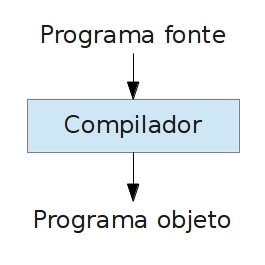
\includegraphics[width=0.25\textwidth]{figuras/compilador}
  \end{center}
  \caption{Estrutura de um compilador}
  \label{fig:compilador}
\end{figure}

\begin{figure}[htp]
  \begin{center}
    
\includegraphics[width=0.6\textwidth]{figuras/interpretador}
  \end{center}
  \caption{Estrutura de um interpretador}
  \label{fig:interpretador}
\end{figure}

Internamente, ambos os programas s\ao\ semelhantes, como explica \cite{Aho08}, que ser\ao\ expostos a seguir.

\subsubsection{An\ah lise l\eh xica}
\subsubsection{An\ah lise sint\ah tica}
\subsubsection{An\ah lise sem\^antica}
\subsubsection{Gera\ca o de c\oh digo intermedi\ah rio}
\subsubsection{Otimiza\ca o}
\subsubsection{Gera\ca o de c\oh digo objeto}
\subsubsection{Ambiente de execu\ca o}

\section{T\oh picos sobre otimiza\ca o}
\subsection{JIT - \emph{Just-in-Time Compilation}}

\section{LLVM - Low Level Virtual Machine}
\subsection{Hist\oh ria}
\subsection{Motiva\ca o}
\subsection{Trabalhos derivados}
\subsection{Otimiza\ca o em m\'ultiplos passos}
